\section{Horshoe Orbit}\label{sec:1d}
To find the initial conditions for the asteroid in a horseshoe orbit, one can initialise the orbit without a velocity, in the vicinity of L3. The coordinates of L3 for the given configuration, are: $[-1,000, 0]$\cite{lecture_notes}.
A time-span of 500000 iterations was used. This results in the following horseshoe orbit:
\begin{figure}[H]
    \centering
    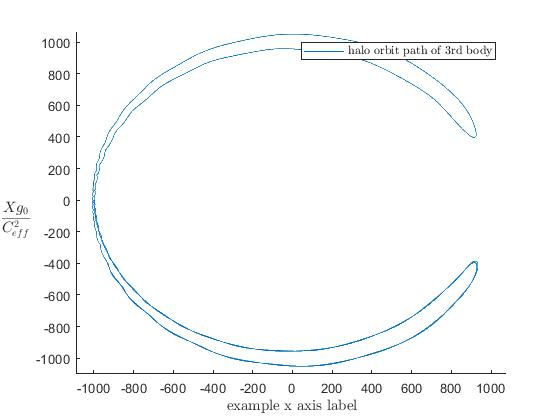
\includegraphics[width=1\textwidth]{Images/plot_1d.jpg}
    \caption{Horseshoe orbit starting near L3}
\end{figure}

\begin{figure}[H]
    \centering
    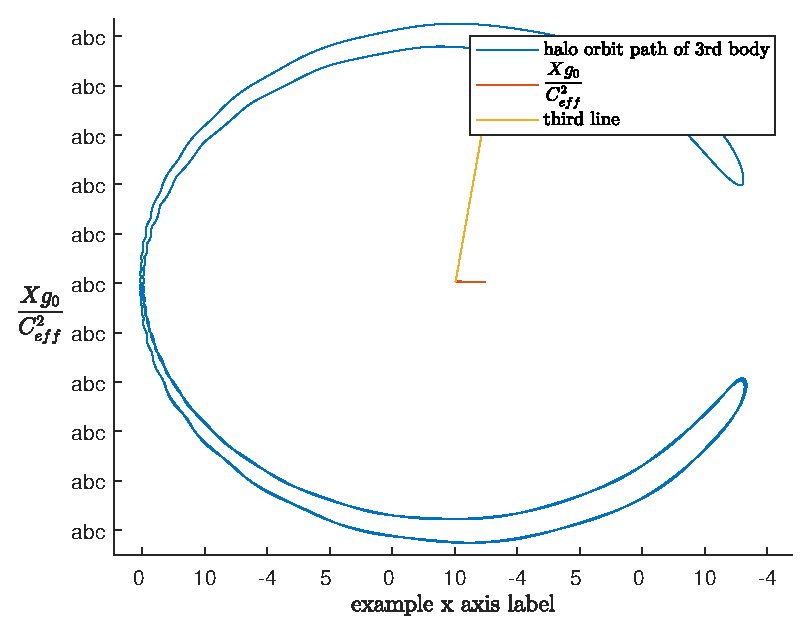
\includegraphics[width=1\textwidth]{Images/plot_1d.eps}
    \caption{Figure consisting of multiple dataseries.}
\end{figure}